\documentclass[a4paper,10pt]{article}
\usepackage[utf8x]{inputenc}
\usepackage{ucs}
\usepackage[english]{babel}
\usepackage[T1]{fontenc}
\usepackage{amsmath}
\usepackage{amsfonts}
\usepackage{amssymb}
\usepackage{bbm}
\usepackage{color}
\usepackage{esint}
\usepackage{hyperref}
\usepackage{pgfplots}
\usepackage{textcomp}
\usepackage{tikz}
\usepackage{tikz-3dplot}
\usepackage{verbatim}

\usetikzlibrary{angles,patterns,quotes}

\title{Electromagnetism}
\author{Nicolas Iooss}

\newcommand{\vF}{\ensuremath\vec{F}} % Force field
\newcommand{\vE}{\ensuremath\vec{E}} % Electric field
\newcommand{\vB}{\ensuremath\vec{B}} % Magnetic field

% Partial derivatives
\newcommand{\pderiv}[2]{\ensuremath\frac{\partial #2}{\partial #1}}
\newcommand{\pdx}[1]{\ensuremath\pderiv{x}{#1}}
\newcommand{\pdxsq}[1]{\ensuremath\pderiv{x^2}{^2 #1}}
\newcommand{\pdy}[1]{\ensuremath\pderiv{y}{#1}}
\newcommand{\pdysq}[1]{\ensuremath\pderiv{y^2}{^2 #1}}
\newcommand{\pdz}[1]{\ensuremath\pderiv{z}{#1}}
\newcommand{\pdzsq}[1]{\ensuremath\pderiv{z^2}{^2 #1}}
\newcommand{\pdt}[1]{\ensuremath\pderiv{t}{#1}}
\newcommand{\pdtsq}[1]{\ensuremath\pderiv{t^2}{^2 #1}}
\newcommand{\pdr}[1]{\ensuremath\pderiv{r}{#1}}
\newcommand{\pdth}[1]{\ensuremath\pderiv{\theta}{#1}}
\newcommand{\pdph}[1]{\ensuremath\pderiv{\varphi}{#1}}

\begin{document}
\maketitle

\section*{Introduction}

This document presents a summary of electromagnetism concepts.

\section{SI units}

The International System of Units (``SI'') defines units in order to measure dimensions, a phenomenon, etc.

\begin{itemize}
  \item A time is measured in seconds: s
  \item A distance is measured in meters: m
  \item A speed is measured in meters per second: m.s\textsuperscript{-1}
  \item An acceleration is measured in meters per second square: m.s\textsuperscript{-2}
  \item A mass is measured in kilograms: kg
  \item A force is measured in newtons: N = kg.m.s\textsuperscript{-2}
  \item The work of a force has the same unit of an energy and is measured in joules: J = kg.m\textsuperscript{2}.s\textsuperscript{-2}
  \item A power is measured in watts: W = J.s\textsuperscript{-1} = kg.m\textsuperscript{2}.s\textsuperscript{-3}
  \item An electric current has an intensity measured in amperes: A
  \item An electric charge is measured in coulombs: C = s.A
  \item An electric power is also measured in watts: W = V.A
  \item A voltage is measured in volts: V = kg.m\textsuperscript{2}.s\textsuperscript{-3}.A\textsuperscript{-1}
  \item An electric impedance is measured in ohms: $\Omega$ = V.A\textsuperscript{-1} = kg.m\textsuperscript{2}.s\textsuperscript{-3}.A\textsuperscript{-2}
  \item An electric capacity is measured in farads: F = kg\textsuperscript{-1}.m\textsuperscript{-2}.s\textsuperscript{4}.A\textsuperscript{2}
  \item An electric inductance is measured in henries: H = kg.m\textsuperscript{2}.s\textsuperscript{-2}.A\textsuperscript{-2}
  \item An electric field (it may be the gradient of a voltage) is measured in volts per meter: V.m\textsuperscript{-1} = kg.m.s\textsuperscript{-3}.A\textsuperscript{-1}
  \item A magnetic field is measured in teslas: T = kg.s\textsuperscript{-2}.A\textsuperscript{-1}
  \item A magnetic flux is measured in webers: Wb = T.m\textsuperscript{2} = V.s = J.A\textsuperscript{-1} = kg.m\textsuperscript{2}.s\textsuperscript{-2}.A\textsuperscript{-1}
\end{itemize}

There exists other units:

\begin{itemize}
  \item A maxwell is: 1 Mx = 10\textsuperscript{-8} Wb
  \item A gauss is: 10\textsuperscript{-4} T
  \item A calory is: 1 cal = 4.1868 J
  \item A mole is: 1 mol = $N_A = 6.022 \times 10^{23}$ (Avogadro's Number)
\end{itemize}

In order to compare values:
\begin{itemize}
  \item Earth's magnetic field is $B_{earth} \approx 10^{-4}$ T = 100 \textmu T
  \item The speed of light is $c = 2.99792458 \times 10^8$ m.s\textsuperscript{-1}
  \item The light from the sun has an intensity of about 1 kW.m\textsuperscript{-2}
  \item The charge of a proton is $e = 1.602 \times 10^{-19}$ C
\end{itemize}

\section{Lorentz force}

When a particle of charge $q$ moves with velocity $\vec{v}$ in an electric field $\vE$ and a magnetic field $\vB$, it will experience a force:
\begin{equation}
  \vF = q \vE + q\vec{v} \times \vB
\end{equation}

Where
\begin{itemize}
  \item $\vF$ is a force in Newton (N = kg.m.s\textsuperscript{-2})
  \item $\vec{v}$ is the velocity in meters per second (m.s\textsuperscript{-1})
  \item $q$ is an electric charge in coulombs (C = s.A)
  \item $\vE$ is the electric field in volts per meter (V.m\textsuperscript{-1} = kg.m.s\textsuperscript{-3}.A\textsuperscript{-1})
  \item $\vB$ is the magnetic field in Tesla (T = kg.s\textsuperscript{-2}.A\textsuperscript{-1})
\end{itemize}

\section{Maxwell equations}

\subsection{Nabla symbol}

Nabla symbol, $\nabla$, is used as a spatial derivation notation to represent several spatial operations, either on a spatial function $f$ or on a spatial vector field $\vec{v}$:

\begin{itemize}
  \item Gradient ``$\nabla f$'' ($\vec{\text{grad}}\left(f\right)$ in French)
     \begin{equation}
       \forall \vec{u}, \left(\nabla f\right) \cdot \vec{u} = D_{\vec{u}} f
     \end{equation}
  \item Divergence ``$\nabla \cdot \vec{v}$'' ($\text{div}\left(\vec{v}\right)$ in French)
     \begin{equation}
       \nabla \cdot \vec{v} = \lim_{|V| \to 0} \iint_{S(V)} \frac{\vec{v} \cdot \vec{n}}{|V|} dS
     \end{equation}
     where $V$ is a volume containing the point where the divergence is taken, $S(V)$ the surface of this volume and $\vec{n}$ a normal vector of the surface.
  \item Curl ``$\nabla \times \vec{v}$'' ($\vec{\text{rot}}\left(\vec{v}\right)$ in French)
     \begin{equation}
       \forall \vec{n},
       \left(\nabla \times \vec{v}\right) \cdot \vec{n} = \lim_{|A| \to 0}\left( \frac{1}{|A|}\oint_{C} \vec{v} \cdot d\vec{r}\right)
     \end{equation}
     where $A$ is an area whose normal is $\vec{n}$ and $C$ is the oriented border of $(A, \vec{n})$.
\end{itemize}

From these definitions, the Laplace operator ``$\Delta f$'' is defined as the divergence of the gradient:

\begin{equation}
  \Delta f = \nabla^2 f = \nabla \cdot \nabla f
\end{equation}

\subsubsection{Cartesian definition}

Given a 3-dimensional Cartesian spatial function $f(x, y, z)$:

\begin{eqnarray}
  \nabla f &=& \left(\begin{array}{c} \pdx{f} \\ \pdy{f} \\ \pdz{f} \end{array}\right)
    = \pdx{f}\vec{e_x} + \pdy{f} \vec{e_y} + \pdz{f} \vec{e_z} \\
  \Delta f = \nabla^2 f& =& \pdxsq{f} + \pdysq{f} + \pdzsq{f}
\end{eqnarray}

Given a 3-dimensional Cartesian spatial vector field $\vec{v}(x, y, z)$:

\begin{eqnarray}
  \nabla \cdot \vec{v} &=& \pdx{v_x} + \pdy{v_y} + \pdz{v_z} \\
  \nabla \times \vec{v} &=& \left(\begin{array}{c}
    \pdy{v_z} - \pdz{v_y} \\
    \pdz{v_x} - \pdx{v_z} \\
    \pdx{v_y} - \pdy{v_x}
    \end{array}\right) \\
  \nabla &=& \left(\begin{array}{c} \pdx{} \\ \pdy{} \\ \pdz{} \end{array}\right) \\
  \nabla^2 \vec{v} &=&
    \left(\begin{array}{c}
      \pdxsq{} + \pdysq{} + \pdzsq{} \\
      \pdxsq{} + \pdysq{} + \pdzsq{} \\
      \pdxsq{} + \pdysq{} + \pdzsq{}
    \end{array}\right) \cdot \left(\begin{array}{c}
      v_x \\
      v_y \\
      v_z
    \end{array}\right)
\end{eqnarray}

$\nabla^2$ is the vector Laplacian.

In this coordinate system, it can be easily shown that:
\begin{eqnarray}
  \nabla \times (\nabla f) &=& 0 \\
  \nabla \cdot (\nabla \times \vec{v}) &=& 0 \\
  \nabla \times (\nabla \times \vec{v}) &=& \nabla(\nabla \cdot \vec{v}) - \nabla^2 \vec{v}
\end{eqnarray}

\subsubsection{Cylindrical definition}

Cylindrical coordinates $(r, \theta, z)$ are defined by:
\begin{eqnarray}
  x &=& r \cos\theta \\
  y &=& r \sin\theta
\end{eqnarray}

\begin{figure}[h]
  \centering
  \tdplotsetmaincoords{64}{110}
  \begin{tikzpicture}[scale=4, tdplot_main_coords,
      axis/.style={->,blue,thick},
      vector/.style={-stealth,red,very thick},
      vector guide/.style={dashed,red,thick}]

    \coordinate (O) at (0,0,0);
    \draw[axis] (0,0,0) -- (1,0,0) node[anchor=north east]{$x$};
    \draw[axis] (0,0,0) -- (0,1,0) node[anchor=west]{$y$};
    \draw[axis] (0,0,0) -- (0,0,1) node[anchor=south]{$z$};

    \pgfmathsetmacro{\Prho}{.9}
    \pgfmathsetmacro{\Ptheta}{40}
    \pgfmathsetmacro{\Pphi}{60}
    \pgfmathsetmacro{\Pr}{\Prho * sin(\Ptheta)}
    \tdplotsetcoord{P}{\Prho}{\Ptheta}{\Pphi}

    \draw[vector] (O) -- (P);
    \draw[vector guide] (O) -- (Pxy) node[color=black,anchor=west,midway]{$r$};
    \draw[vector guide] (Pxy) -- (P);
    \draw[vector guide] (P) -- (Pz);
    \draw (Pz) node[color=black,anchor=east]{$z$};

    \tdplotdrawarc{(O)}{.3}{0}{\Pphi}{anchor=north}{$\theta$}
    \tdplotdrawarc[dashed]{(O)}{\Pr}{0}{360}{}{}
    \tdplotdrawarc[dashed]{(Pz)}{\Pr}{0}{360}{}{}

    \tdplotsetrotatedcoords{\Pphi}{0}{0}
    \tdplotsetrotatedcoordsorigin{(P)}
    \draw[thick,tdplot_rotated_coords,->] (0,0,0)
      -- (.3,0,0) node[anchor=west]{$\vec{e_r}$};
    \draw[thick,tdplot_rotated_coords,->] (0,0,0)
      -- (0,.3,0) node[anchor=west]{$\vec{e_\theta}$};
    \draw[thick,tdplot_rotated_coords,->] (0,0,0)
      -- (0,0,.3) node[anchor=south]{$\vec{e_z}$};
  \end{tikzpicture}
  \caption{Cylindrical coordinates}
\end{figure}

With a spatial function $f(r, \theta, z)$ and a spatial vector field $\vec{v}(r, \theta, z)$:
\begin{eqnarray}
  \nabla f &=& \pdr{f}\vec{e_r} + \frac{1}{r}\pdth{f} \vec{e_\theta} + \pdz{f} \vec{e_z} \\
  \nabla \cdot \vec{v} &=& \frac{1}{r}\pdr{(r v_r)} + \frac{1}{r}\pdth{v_\theta} + \pdz{v_z} \\
  \nabla \times \vec{v} &=&
    \left(\begin{array}{c}
      \frac{1}{r}\pdth{v_z} - \pdz{v_\theta} \\
      \pdz{v_r} - \pdr{v_z} \\
      \frac{1}{r}\left(\pdr{(r v_\theta)} - \pdth{v_r}\right)
    \end{array}\right)
\end{eqnarray}

\subsubsection{Spherical definition}

Spherical coordinates $(r, \theta, \varphi)$ are defined by:
\begin{eqnarray}
  x &=& r \sin\theta \cos\varphi \\
  y &=& r \sin\theta \sin\varphi \\
  z &=& r \cos\theta
\end{eqnarray}

$r$ is the radial distance, $\varphi$ is the azimuthal angle and $\theta$ is the polar angle.

\begin{figure}[h]
  \centering
  \tdplotsetmaincoords{60}{110}
  \begin{tikzpicture}[scale=4, tdplot_main_coords,
      axis/.style={->,blue,thick},
      vector/.style={-stealth,red,very thick},
      vector guide/.style={dashed,red,thick}]

    \coordinate (O) at (0,0,0);
    \draw[axis] (0,0,0) -- (1,0,0) node[anchor=north east]{$x$};
    \draw[axis] (0,0,0) -- (0,1,0) node[anchor=west]{$y$};
    \draw[axis] (0,0,0) -- (0,0,1) node[anchor=south]{$z$};

    \pgfmathsetmacro{\Pr}{.8}
    \pgfmathsetmacro{\Ptheta}{30}
    \pgfmathsetmacro{\Pphi}{60}
    \tdplotsetcoord{P}{\Pr}{\Ptheta}{\Pphi}

    \draw[vector] (O) -- (P) node[color=black,below,midway]{$r$};
    \draw[vector guide] (O) -- (Pxy) -- (P) -- (Pz);

    \tdplotdrawarc{(0,0,0)}{.3}{0}{\Pphi}{anchor=north}{$\varphi$}
    \tdplotsetthetaplanecoords{\Pphi}
    \tdplotdrawarc[tdplot_rotated_coords]{(0,0,0)}{.3}{0}{\Ptheta}{anchor=south}{$\theta$}

    \draw[dashed,tdplot_rotated_coords] (\Pr,0,0) arc (0:90:\Pr);
    \draw[dashed] (\Pr,0,0) arc (0:90:\Pr);

    \tdplotsetrotatedcoords{\Pphi}{\Ptheta}{0}
    \tdplotsetrotatedcoordsorigin{(P)}
    \draw[thick,tdplot_rotated_coords,->] (0,0,0)
      -- (.3,0,0) node[anchor=west]{$\vec{e_\theta}$};
    \draw[thick,tdplot_rotated_coords,->] (0,0,0)
      -- (0,.3,0) node[anchor=west]{$\vec{e_\varphi}$};
    \draw[thick,tdplot_rotated_coords,->] (0,0,0)
      -- (0,0,.3) node[anchor=south]{$\vec{e_r}$};
  \end{tikzpicture}
  \caption{Spherical coordinates}
\end{figure}

With a spatial function $f(r, \theta, \varphi)$ and a spatial vector field $\vec{v}(r, \theta, \varphi)$:
\begin{eqnarray}
  \nabla f &=& \pdr{f}\vec{e_r} + \frac{1}{r}\pdth{f}\vec{e_\theta} + \frac{1}{r \sin\theta}\pdph{f}\vec{e_\varphi} \\
  \nabla \cdot \vec{v} &=& \frac{1}{r^2}\pdr{r^2 v_r} + \frac{1}{r \sin\theta}\pdth{v_\theta \sin\theta} + \frac{1}{r\sin\theta}\pdph{v_\varphi} \\
  \nabla \times \vec{v} &=& \left(\begin{array}{c}
    \frac{1}{r \sin\theta}\left(\pdth{v_\varphi \sin\theta} - \pdph{v_\theta}\right) \\
    \frac{1}{r}\left(\frac{1}{\sin\theta}\pdph{v_r} - \pdr{(r v_\varphi)}\right) \\
    \frac{1}{r}\left(\pdr{(r v_\theta)} - \pdth{v_r}\right)
    \end{array}\right)
\end{eqnarray}

\subsubsection{Link between non-local operations and local Nabla operators}

The Divergence theorem (also known as Gauss's theorem or Green-Ostrogradski's theorem):
\begin{quote}
  Given a volume $V$ having a surface $S(V) = \partial V$ (and $\vec{n}$ being the local normal of surface element $dS$ directed outside of $V$),
  \begin{equation}
    \iiint_V \nabla \cdot \vec{v} dV = \oiint_{S(V)} \vec{v} \cdot \vec{n}dS
  \end{equation}
\end{quote}

Kelvin-Stokes theorem (also known as the fundamental theorem for curls):
\begin{quote}
  In a 3-dimensional space, given an oriented closed circuit $C$ and an oriented smooth area $A$ which is bordered by $C = \partial A$,
  \begin{equation}
    \iint_A (\nabla \times \vec{v}) \cdot \vec{n}dS = \oint_C \vec{v} \cdot \vec{dr}
  \end{equation}
\end{quote}

\subsection{Maxwell's equations in the void}

In the void (in the absence of magnetic or polarizable media):
\begin{eqnarray}
  \text{Gauss's law: } \nabla \cdot \vE &=& \frac {\rho} {\varepsilon_0} \\
  \text{Gauss's law for magnetism: } \nabla \cdot \vB &=& 0 \\
  \text{Faraday's law of induction: } \nabla \times \vE &=& -\pdt{\vB} \\
  \text{Ampère's circuital law: } \nabla \times \vB &=& \mu_0\left(\vec{j} + \varepsilon_0 \pdt{\vE}\right)
\end{eqnarray}

Where
\begin{itemize}
  \item $\varepsilon_0 \approx 8.854187817 \times 10^{-12} F.m^{-1}$ is the vacuum permittivity, in farads per meter (= kg\textsuperscript{-1}.m\textsuperscript{-3}.s\textsuperscript{4}.A\textsuperscript{2})
  \item $\mu_0 = 4\pi \times 10^{-7} N.A^{-2} \approx 1.2566370614 \times 10^{-6} H.m^{-1}$ is the vacuum permeability, in henries per meter (= kg.m.s\textsuperscript{-2}.A\textsuperscript{-2})
  \item $\rho$ is the local electric charge density in coulombs per meter cube (C.m\textsuperscript{-3} = m\textsuperscript{-3}.s.A)
  \item $\vec{j}$ is the current density in amperes per meter square (A.m\textsuperscript{-2})
  \item $\vE$ is the electric field in volts per meter (V.m\textsuperscript{-1} = kg.m.s\textsuperscript{-3}.A\textsuperscript{-1})
  \item $\vB$ is the magnetic field in Tesla (T = kg.s\textsuperscript{-2}.A\textsuperscript{-1} = H.A.m\textsuperscript{-2})
\end{itemize}

When the fields are static, $\vE$ is a conservative field. This means that it is the gradient of an electric potential:
\begin{equation}
  \vE = -\nabla V
\end{equation}

This is linked to the fact that along a curve between two points $A$ and $B$ with potentials $V_A$ and $V_B$:
\begin{equation}
  V_A - V_B = \int_A^B \vE.\vec{dr}
\end{equation}

\subsection{Maxwell's equations}

Sometimes the Magnetic Field Strength $H$ is used instead of $B$.
In the void, $H = \frac{B}{\mu_0}$.
In magnetic materials characterized by an internal magnetic field $M$:
\begin{equation}
  B = \mu_0 (H + M)
\end{equation}

With an isotropic linear magnetic medium, $B = \mu H$.

With polarized materials:
\begin{equation}
  D = \varepsilon_0 E + P
\end{equation}

With an isotropic linear dielectric material, $D = \varepsilon E$.

Maxwell's equations become:
\begin{eqnarray}
  \text{Gauss's law: } \nabla \cdot \vec{D} &=& \rho \\
  \text{Gauss's law for magnetism: } \nabla \cdot \vB &=& 0 \\
  \text{Faraday's law of induction: } \nabla \times \vE &=& -\pdt{\vB} \\
  \text{Ampère's circuital law: } \nabla \times \vec{H} &=& \vec{j} + \pdt{\vec{D}}
\end{eqnarray}

\subsection{EM wave propagation in the vacuum}

In the vacuum, there is no local charge: $\rho = 0$ and $\vec{j} = 0$. 

\begin{eqnarray*}
  \nabla^2 \vE &=& \nabla(\nabla \cdot \vE) - \nabla \times (\nabla \times \vE) \\
               &=& \nabla(0) + \nabla \times \pdt{\vB} \\
               &=& \pdt{(\nabla \times \vB)} \text{ because $\vB$ is supposed smooth} \\
               &=& \pdt{}\left(\mu_0 \varepsilon_0 \pdt{\vE}\right) \\
  \nabla^2 \vE &=& \mu_0 \varepsilon_0 \pdtsq{\vE}
\end{eqnarray*}

The solutions of these linear differential equations describe electromagnetic waves such as the propagation of light in the vacuum.

Some of them are linear combinations of waves defined by the following equations:
\begin{eqnarray}
  \vE &=& \vE_0 \sin\left(-\omega t + \vec{k} \cdot \vec{r}\right) \\
  \vB &=& \vB_0 \sin\left(-\omega t + \vec{k} \cdot \vec{r}\right) \\
  \vec{k} \times \vE_0 &=& \omega \vB_0 \\
  \vec{k} \times \vB_0 &=& -\omega \mu_0 \varepsilon_0 \vE_0
\end{eqnarray}

Therefore:
\begin{eqnarray}
  k = |\vec{k}| &=& \omega \sqrt{\mu_0 \varepsilon_0}
\end{eqnarray}

These equations describe a linearly polarized monochromatic electromagnetic plane wave, where $\vec{k}$, $\vE_0$ and $\vB_0$ are orthogonal.
Its phase speed, which is the speed of the light is:
\begin{equation}
  c = \frac{w}{k} = \frac{1}{\sqrt{\mu_0 \varepsilon_0}} \approx 2.99792458 \times 10^8 \text{m.s}^{-1}
\end{equation}

Then:
\begin{eqnarray}
  E &=& \left|\vE\right| = \frac{\omega}{k} \left|\vB\right| = c B \\
  B &=& \frac{E}{c}
\end{eqnarray}

\subsubsection{Poynting vector}

Electromagnetic waves are able to transport energy from transmitter to receiver.
The Poynting vector describes this: its direction is the direction of propagation and its amplitude is the transmitted power (in watts per meter square):
\begin{equation}
  \vec{S} = \frac{1}{\mu_0} \vE \times \vB
\end{equation}

For a polarized monochromatic plane wave, $\vec{S}$ and $\vec{k}$ are aligned and:
\begin{equation}
  \left|\vec{S}\right| = \frac{1}{\mu_0} E B = \frac{c}{\mu_0} B^2 = \frac{1}{c\mu_0} E^2
\end{equation}

The amplitude of the Poynting vector oscillates too:
\begin{equation}
  \left|\vec{S}\right| = S_0 \sin^2\left(-\omega t + \vec{k} \cdot \vec{r}\right)
\end{equation}

The \emph{intensity} of the wave is the average of this amplitude (in W.m\textsuperscript{-2}):
\begin{equation}
  I_{wave} = \bar{S} = \frac{S_0}{2} = \frac{c}{\mu_0} B_{rms}^2 = \frac{1}{c\mu_0} E_{rms}^2
\end{equation}

RMS means « Root Mean Square »: $E_{rms} = \frac{1}{\sqrt{2}} E_0$.

The intensity of a wave can be used to compute the radiation pressure, which is the force caused by the momentum that is carried by the wave when it is absorbed by a surface (if the wave is reflected, this force is multiplied by 2):
\begin{equation}
  F = \frac{\Delta p}{\Delta t} = \frac{\Delta \text{energy}}{c \Delta t} = \frac{\text{power}}{c} =  \frac{I_{wave} A_{surface}}{c}
\end{equation}

\section{Theoretical examples}

\subsection{Punctual charge}

A punctual charge $q$ emits an electric field and does not emit a magnetic field.
The spherical symmetry of the charge leads to an electric fields which only has a radial component in spherical coordinates.

\begin{figure}[h]
  \centering
  \begin{tikzpicture}
    \node[fill,circle,shading=ball,ball color=red] (q) at (0,0) {};
    \node at (0,-.5) {$q$};
    \node[inner sep=0] (P) at (2,0) {};

    \draw[dashed] (q) circle (2);
    \draw[dashed] (q) -- node[below,midway]{$r$} (P);
    \draw[red,->] (P) -- +(3,0) node[above,midway]{$\vE = E_r \vec{e_r}$};
  \end{tikzpicture}
  \caption{Electric field of a punctual charge}
\end{figure}

Integrating on a sphere (using Gauss's law) leads to the following equations:

\begin{eqnarray}
  \vE(r, \theta, \varphi) &=& \frac{q}{4 \pi \varepsilon_0 r^2} \vec{e_r} \\
  \vB &=& 0
\end{eqnarray}

This leads to the force that a charge $q_1$ exerts on another one, $q_2$:

\begin{equation}
  \vF_{q1 \rightarrow q2} = \frac{q_1 q_2}{4 \pi \varepsilon_0 r^2} \vec{e}_{q1q2}
\end{equation}

The electric field of a punctual charge is the gradient of the following voltage (to a constant):
\begin{equation}
  V_q = \frac{1}{4 \pi \varepsilon_0} \frac{q}{r}
\end{equation}

\subsubsection{Coulomb's law}

The contribution $\vec{dE}$ of an infinitesimal charge $dq$ is in spherial coordinates:
\begin{equation}
  \text{Coulomb's law: }\vec{dE}(r, \theta, \varphi) = \frac{dq}{4 \pi \varepsilon_0 r^2} \vec{e_r} = \frac{dq}{4 \pi \varepsilon_0 r^3} \vec{r}
\end{equation}

This is a direct consequence of the electric field of a punctual charge.

\subsection{Dipole}

An electric dipole consists in a pair of opposite charges, $\pm q$, separated by a small distance $d$.
With $N$ and $P$ being the points with the negative and positive charges, the value of the dipole is defined as:
\begin{equation}
  \vec{p} = q\vec{d} \text{ with }\vec{d} = \overrightarrow{NP}
\end{equation}

The resulting electric field is the superposition of the fields of the two punctual charges.
For a point at distance $r_+$ of $P$ and $r_-$ of $N$, the electric potential at the point can be computed as:

\begin{eqnarray}
  V &=& \frac{1}{4 \pi \varepsilon_0} \left(\frac{q}{r_+} - \frac{q}{r_-}\right) \\
    &=& \frac{q}{4 \pi \varepsilon_0} \frac{r_- - r_+}{r_+ r_-}
\end{eqnarray}

Let $r$ be the distance between the point and the middle of the dipole, and $\theta$ the andle relative to $\vec{p}$.

\begin{figure}[h]
  \centering
  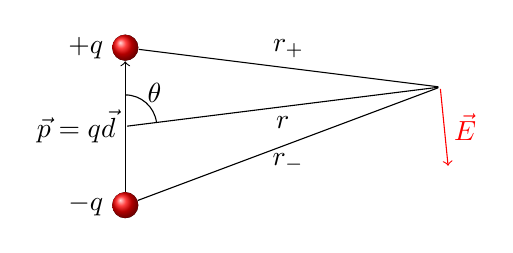
\begin{tikzpicture}
    \node[fill,circle,shading=ball,ball color=red] (P) at (0,1) {};
    \node[fill,circle,shading=ball,ball color=red] (N) at (0,-1) {};
    \node[inner sep=0] (O) at (0,0) {};
    \node at (-.5,1) {$+q$};
    \node at (-.5,-1) {$-q$};
    \node[inner sep=0] (A) at (4,.5) {};

    \draw[->] (N) -- (P) node[midway,anchor=east] {$\vec{p} = q\vec{d}$};
    \draw (P) -- (A) node[midway,anchor=south] {$r_+$};
    \draw (O) -- (A) node[midway,anchor=north] {$r$};
    \draw (N) -- (A) node[midway,anchor=north] {$r_-$};
    \draw[red,->] (A) -- +(.1,-1) node[midway,anchor=west] {$\vE$};

    \draw pic[draw=black,"$\theta$",angle eccentricity=1.4,angle radius=4mm] {angle=A--O--P};
  \end{tikzpicture}
  \caption{Electric field of a dipole}
\end{figure}

The trigonometry states that:
\begin{eqnarray}
  r &=& \frac{d}{2} \cos\theta + \sqrt{r_+^2 - \left(\frac{d}{2} \sin\theta\right)^2} \\
  r &=& \frac{d}{2} \cos\left(\pi-\theta\right) + \sqrt{r_-^2 - \left(\frac{d}{2} \sin\left(\pi-\theta\right)\right)^2}
\end{eqnarray}

Therefore:
\begin{eqnarray}
  r_+ &=& \sqrt{\left(r - \frac{d}{2} \cos\theta\right)^2 + \left(\frac{d}{2} \sin\theta\right)^2} = \sqrt{r^2 - rd\cos\theta + \frac{d^2}{4}} \\
  r_- &=& \sqrt{\left(r + \frac{d}{2} \cos\theta\right)^2 + \left(\frac{d}{2} \sin\theta\right)^2} = \sqrt{r^2 + rd\cos\theta + \frac{d^2}{4}}
\end{eqnarray}

When $d << r$, at the first order,
\begin{eqnarray}
  r_+ &=& r\left(1 - \frac{d}{2r}\cos\theta + o\left(\frac{d}{r}\right)\right) = r - \frac{d}{2}\cos\theta + o(d) \\
  r_- &=& r + \frac{d}{2}\cos\theta + o(d) \\
  r_- - r_+ &=& d\cos\theta + o(d) \\
  r_+ r_- &=& r^2\left(1 + o\left(\frac{d}{r}\right)\right) \\
  \frac{1}{r_+ r_-} &=& \frac{1}{r^2}\left(1 + o\left(\frac{d}{r}\right)\right) \\
  \frac{r_- - r_+}{r_+ r_-} &\approx& \frac{d}{r^2}\cos\theta
\end{eqnarray}

The electric potential of the dipole is therefore at long range:
\begin{equation}
  V_{dipole}(r, \theta) \approx \frac{qd}{4 \pi \varepsilon_0 r^2}\cos\theta = \frac{1}{4 \pi \varepsilon_0 r^2}\vec{p}.\vec{e_r}
\end{equation}

Using spherical coordinates with the dipole aligned on the $z$ axis, the electric field of the dipole is:
\begin{eqnarray}
  \vE_{dipole}(r, \theta, \varphi) &=& -\nabla V = \frac{qd}{2 \pi \varepsilon_0 r^3}\cos\theta \vec{e_r} + \frac{qd}{4 \pi \varepsilon_0 r^3}\sin\theta \vec{e_\theta} \\
    &=& \frac{qd}{4 \pi \varepsilon_0 r^3} \left(2\cos\theta \vec{e_r} + \sin\theta \vec{e_\theta}\right)
\end{eqnarray}

The lines of equipotential are defined by $r = \sqrt{\frac{qd}{4 \pi \varepsilon_0 V_{line}}\cos\theta}$ for a non-null potential, $\theta = \frac{\pi}{2}$ otherwise.

In order to represent in cut-off plan where the dipole is at the origin and aligned with the $z$ axis, and the other axis is $y$, here are some equations:
\begin{eqnarray}
  \theta &\in& [0, \pi] \\
  z &=& r \cos\theta \\
  y &=& r \sin\theta \geq 0 \\
  r &=& \sqrt{\frac{qd}{4 \pi \varepsilon_0 V_{line}}\cos\theta}
\end{eqnarray}

An equipotential line $V = V_{line}$ then depends on a constant $r_l = \sqrt{\frac{qd}{4 \pi \varepsilon_0 V_{line}}}$.

\begin{eqnarray}
  r &=& r_l \sqrt{\cos\theta} \\
  z &=& r_l (\cos\theta)^{3/2} \\
  \cos\theta &=& \left(\frac{z}{r_l}\right)^{2/3} \\
  r &=& r_l \left(\frac{z}{r_l}\right)^{1/3} \\
  y &=& \sqrt{r^2 - z^2} = r_l \sqrt{\left(\frac{z}{r_l}\right)^{4/3} - \left(\frac{z}{r_l}\right)^2}
\end{eqnarray}

The equipotential lines are dilatations of the following curve (with $y = r_l Y$ and $z = r_l Z$):
\begin{eqnarray}
  Y &=& \sqrt{Z^{4/3} - Z^2} \\
  Y &=& Z^{2/3} \sqrt{1 - Z^{4/3}}
\end{eqnarray}

\begin{figure}[h]
  \centering
  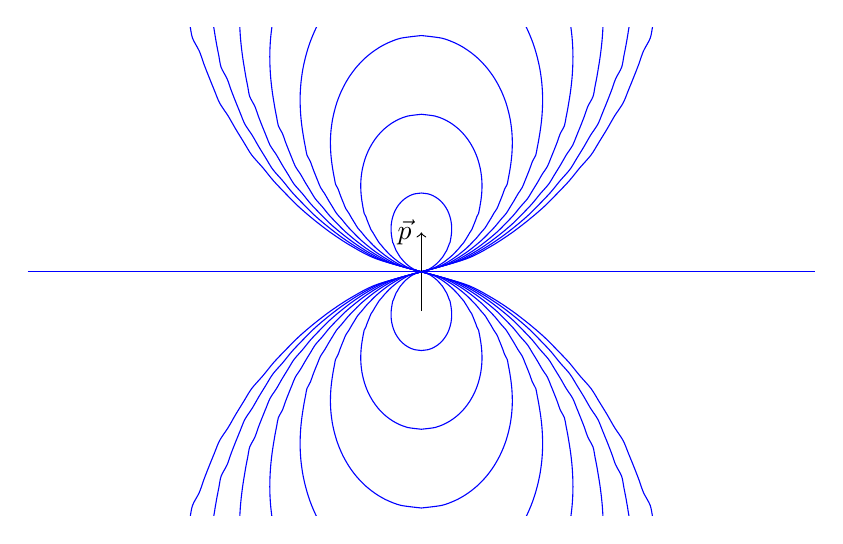
\begin{tikzpicture}
    \draw[->] (0,-.5) -- (0,.5) node[anchor=east] {$\vec{p}$};

    % \z is Z and \r is r_l, so "z" is \r*\z and "y" is \r*Y
    \begin{scope}
      \clip(-5,-3.1) rectangle (5,3.1);
      \draw[blue] (-5,0) -- (5, 0);
      \foreach \r in {1,...,8}
        \draw[scale=1,domain=0:1.01,samples=50,smooth,variable=\z,blue]
          plot ({\r*sqrt(max(0, (\z*\z)^(2/3) - \z*\z))},{\r*min(\z, 1)})
          plot ({-\r*sqrt(max(0, (\z*\z)^(2/3) - \z*\z))},{\r*min(\z, 1)})
          plot ({\r*sqrt(max(0, (\z*\z)^(2/3) - \z*\z))},{-\r*min(\z, 1)})
          plot ({-\r*sqrt(max(0, (\z*\z)^(2/3) - \z*\z))},{-\r*min(\z, 1)});
    \end{scope}
  \end{tikzpicture}
  \caption{Equipotential lines of an electric dipole}
\end{figure}

\subsection{Capacitor}

Let's consider two parallel planes of area $A$ that can be charged with opposite charges $+q$ and $-q$, separated by distance $d$.
Between these planes, a dielectric material has a permittivity $\epsilon = k\epsilon_0$ (with $k \ge 1$).
Let's define a Cartesian coordinate system such that the planes are parallel to $(Oxy)$ and the origin is inbetween the planes.

When analyzing the electromagnetic field between these planes, they can be considered infinite.
With this hypothesis, the symmetry of the system leads to an electric fields which only has a $z$ component.

\begin{figure}[h]
  \centering
  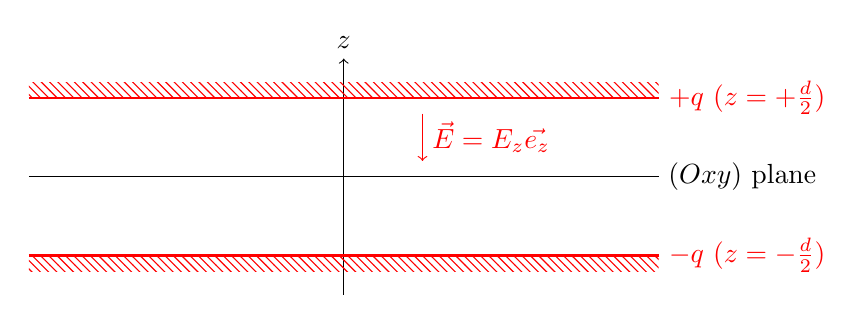
\begin{tikzpicture}
    \draw (-4,0) -- (4,0) node[anchor=west] {$(Oxy)$ plane};
    \draw[->] (0,-1.5) -- (0,1.5) node[anchor=south] {$z$};

    \draw[thick,red] (-4,1) -- (4,1) node[anchor=west] {$+q$ ($z = +\frac{d}{2}$)};
    \draw[thick,red] (-4,-1) -- (4,-1) node[anchor=west] {$-q$ ($z = -\frac{d}{2}$)};
    \draw[draw=none, pattern=north west lines, pattern color=red] (-4,1) rectangle (4,1.2);
    \draw[draw=none, pattern=north west lines, pattern color=red] (-4,-1) rectangle (4,-1.2);

    \draw[red,->] (1,.8) -- (1,.2) node[midway,anchor=west] {$\vE = E_z \vec{e_z}$};
  \end{tikzpicture}
  \caption{Electric field of an infinite capacitor}
\end{figure}

With a surface charge density $\sigma = \frac{q}{A}$, the electric field is:
\begin{equation}
  \vE = -\frac{\sigma}{\varepsilon} \vec{e_z} = -\frac{q}{\varepsilon A} \vec{e_z}
\end{equation}

This is the gradient of the following electric potential:
\begin{equation}
  V(z) = \frac{q}{\varepsilon A} z + V(z=0)
\end{equation}

The voltage between the two planes is:
\begin{equation}
  V = V\left(z=\frac{d}{2}\right) - V\left(z=-\frac{d}{2}\right) = \frac{qd}{\varepsilon A}
\end{equation}

This defines a capacitance $C$ such that $q = CV$:
\begin{eqnarray}
  C &=& \frac{\varepsilon A}{d} \text{ (in farads)} \\
  I &=& C \frac{dV}{dt}
\end{eqnarray}

A capacitor has an electric energy linked with the electric power $VI = CV \frac{dV}{dt}$:
\begin{equation}
  U_e = \frac{CV^2}{2}
\end{equation}

\subsection{Long straight wire}

A long straight wire which carries an electric current $I$ produces a magnetic field $B$ that circles around the wire (there is a cylindrical symmetry).

\begin{figure}[h]
  \centering
  \tdplotsetmaincoords{64}{110}
  \begin{tikzpicture}[tdplot_main_coords]
    \coordinate (O) at (0,0,0);
    \draw[dashed,black] (0,0,0) -- (4,0,0);
    \draw[dashed,black] (0,0,0) -- (0,4,0);
    \draw[thick,red,->] (0,0,-2) -- (0,0,2) node[anchor=south]{$I$};

    \pgfmathsetmacro{\Ptheta}{50}
    \pgfmathsetmacro{\Pr}{3}
    \tdplotsetcoord{P}{\Pr}{90}{\Ptheta}

    \draw (O) -- (Pxy) node[color=black,anchor=west,midway]{$r$};

    \tdplotdrawarc{(O)}{.3}{0}{\Ptheta}{anchor=north}{$\theta$}

    \tdplotsetrotatedcoords{30}{0}{0}
    \foreach \r in {1,...,3} {
      \tdplotdrawarc[tdplot_rotated_coords,blue,->]{(O)}{\r}{0}{90}{}{}
      \tdplotdrawarc[tdplot_rotated_coords,blue,->]{(O)}{\r}{90}{180}{}{}
      \tdplotdrawarc[tdplot_rotated_coords,blue,->]{(O)}{\r}{180}{270}{}{}
      \tdplotdrawarc[tdplot_rotated_coords,blue,->]{(O)}{\r}{270}{360}{}{}
    }

    \tdplotsetrotatedcoords{\Ptheta}{0}{0}
    \tdplotsetrotatedcoordsorigin{(Pxy)}
    \draw[thick,tdplot_rotated_coords,blue,->] (0,0,0)
      -- (0,1,0) node[anchor=west]{$\vec{B}$};
  \end{tikzpicture}
  \caption{Magnetic field of a long wire}
\end{figure}

Using Ampère’s circuital law in cylindrical coordinates:
\begin{equation}
  \vB(r, \theta, z) = \frac{\mu_0 I}{2\pi r} \vec{e_\theta}
\end{equation}

\subsubsection{Biot-Savart law}

The contribution $\vec{dB}$ of an infinitesimal length of conductor $\vec{dL}$ carrying electric current $I$ is in spherial coordinates:
\begin{equation}
  \text{Biot-Savart law: }\vec{dB}(r, \theta, \varphi) = \frac{\mu_0 I}{4 \pi r^2} \vec{dL} \times \vec{e_r}
   = \frac{\mu_0 I}{4 \pi r^3} \vec{dL} \times \vec{r}
\end{equation}

Integrating the Biot-Savart law over the long straight wire in cylindrical coordinates leads to defining a specific coordinate system:
\begin{itemize}
  \item $z$ is the position of the infinitesimal length of conductor along the wire.
  \item $R$ is the distance between the wire and the point where $\vB$ is computed.
  \item $\vec{r}$ is the vector from the integrated point to the point where $\vB$ is computed.
  \item $\alpha$ is the angle between the wire ($z$ axis) and $\vec{r}$.
  \item $\vec{e_\theta}$ is the matching unit vector in cylindrical coordinates for the point where $\vB$ is computed.
\end{itemize}

This allows computing $\vec{dz} \times \vec{r} = (r \sin\alpha)dz \vec{e_\theta}$

\begin{eqnarray}
  \vB(R,\theta,z=0) &=& \int_{-\infty}^{+\infty} \frac{\mu_0 I}{4 \pi r^3} \vec{dz} \times \vec{r} \\
    &=& \frac{\mu_0 I}{4 \pi} \int_{-\infty}^{+\infty} \frac{r \sin\alpha}{r^3} dz \vec{e_\theta} \\
    &=& \frac{\mu_0 I}{4 \pi} \int_{-\infty}^{+\infty} \frac{R}{(R^2 + z^2)^{3/2}} dz \vec{e_\theta} \\
    &=& \frac{\mu_0 I}{4 \pi} \int_{-\infty}^{+\infty} \frac{R}{(R^2 + R^2 Z^2)^{3/2}} RdZ \vec{e_\theta} \\
    &=& \frac{\mu_0 I}{4 \pi R} \int_{-\infty}^{+\infty} \frac{1}{(1 + Z^2)^{3/2}} dZ \vec{e_\theta} \\
  \vB(R,\theta,z=0) &=& \frac{\mu_0 I}{2 \pi R} \vec{e_\theta}
\end{eqnarray}

Because:
\begin{eqnarray}
  \int_{-\infty}^{+\infty} \frac{1}{(1 + Z^2)^{3/2}} dZ &=& 2\int_{0}^{+\infty} \frac{1}{(1 + Z^2)^{3/2}} dZ \\
    &=& 2\int_{0}^{+\infty} \frac{1}{\left(1 + \left(\frac{1}{x}\right)^2\right)^{3/2}} \frac{1}{x^2} dx \\
    &=& 2\int_{0}^{+\infty} \frac{x^3}{\left(x^2 + 1\right)^{3/2}} \frac{1}{x^2} dx \\
    &=& \int_{0}^{+\infty} \frac{2x}{\left(x^2 + 1\right)^{3/2}} dx \\
    &=& \left[-2 \frac{1}{\sqrt{x^2 + 1}}\right]_{0}^{+\infty} \\
   &=& 2
\end{eqnarray}

\subsection{Current loop}

A circle of radius $R$ carries an electric current $I$.
This produces a magnetic field $B$ that looks like a tore around the circle.
Along the axis of the circle, the magnetic field is aligned with the axis and can be computed using Biot-Savart law.

\begin{figure}[h]
  \centering
  \tdplotsetmaincoords{64}{110}
  \begin{tikzpicture}[tdplot_main_coords, scale=2]
    \coordinate (O) at (0,0,0);

    \tdplotsetrotatedcoords{55}{0}{0}
    \tdplotdrawarc[tdplot_rotated_coords,red,thick,->]{(O)}{1}{0}{90}{}{}
    \tdplotdrawarc[tdplot_rotated_coords,red,thick,->]{(O)}{1}{90}{180}{}{}
    \tdplotdrawarc[tdplot_rotated_coords,red,thick,->]{(O)}{1}{180}{270}{}{}
    \tdplotdrawarc[tdplot_rotated_coords,red,thick,->]{(O)}{1}{270}{360}{}{}

    \draw[dashed] (0,0,0) -- (2,0,0);
    \draw[dashed] (0,0,0) -- (0,2,0);
    \draw[->] (0,0,-1) -- (0,0,1) node[anchor=south]{$z$};
    \draw[blue,thick,->] (0,0,.4) -- (0,0,.9) node[anchor=west,midway]{$\vB$};

    \tdplotsetcoord{P}{1}{90}{50}
    \draw[tdplot_rotated_coords] (O) -- (P) node[anchor=north,midway]{$R$};
    \draw[tdplot_rotated_coords,->] (P) -- (0,0,.4) node[anchor=south,midway]{$\vec{r}$};
    \draw (P) node[color=red,anchor=north]{$I$};

    \tdplotdrawarc{(O)}{.3}{0}{50}{anchor=north}{$\theta$}
  \end{tikzpicture}
  \caption{Magnetic field of a current loop along its axis}
\end{figure}

On the axis of the loop:
\begin{eqnarray}
  \vB(z) &=& \oint_{loop} \frac{\mu_0 I}{4 \pi r^3} \vec{dL} \times \vec{r} \\
    &=& \frac{\mu_0 I}{4 \pi r^3} \int_0^{2\pi} R d\theta . R \vec{e_z} \\
    &=& \frac{\mu_0 I R^2}{2 r^3} \vec{e_z} \\
  \vB(z) &=& \frac{\mu_0 I R^2}{2 \left(R^2 + z^2\right)^{3/2}} \vec{e_z}
\end{eqnarray}

At the center of the loop:
\begin{equation}
  \vB_{z=0} = \frac{\mu_0 I}{2R} \vec{e_z}
\end{equation}

Therefore on the axis:
\begin{equation}
  \vB(z) = \left(\frac{R^2}{R^2 + z^2}\right)^{3/2} \vB_{z=0}
\end{equation}

\subsection{Coils}

\subsubsection{Solenoid}

A solenoid is a long straight coil of wire that carries a current.
It generates a nearly uniform magnetic field similar to that of a bar magnet.
If a solenoid consists in $N$ turns over the distance $d$, its \emph{turn density} is $n = \frac{N}{d}$.

Ampere's law computed on a rectangular path between the inner part of the solenoid and the outer one gives a good approximation of the amplitude of the magnetic field:
\begin{equation}
  B = \mu n I
\end{equation}

When the solenoid has an iron core, $\mu = k \mu_0$ and the produced magnetic field is much stronger ($k$ can be several hundreds with some ferromagnetic materials).
This is the basis of an electromagnet.

When the intensity changes, an Electromotive Force (EMF) appears and Faraday's law of induction kicks in:
\begin{equation}
  \nabla \times \vE = -\pdt{\vB}
\end{equation}

When integrating over an area $A$, the magnetic flux is $BA$ and the induced voltage is (for $N$ turns):
\begin{equation}
  V = -N \pdt{(BA)} = -\mu N n A \frac{dI}{dt}
\end{equation}

This defines the inductance $L$ of a solenoid:
\begin{eqnarray}
  L &=& \mu N n A = \frac{\mu N^2 A}{d} \\
  V &=& L \frac{dI}{dt}
\end{eqnarray}

The sign changed because the EMF opposes an applied voltage, in computations done for electric circuits.

A coil has a magnetic energy linked with the electric power $VI = LI \frac{dI}{dt}$:
\begin{equation}
  U_m = \frac{LI^2}{2}
\end{equation}

\subsubsection{Toroid}

When the solenoid is itself curved as a tore, this produces a toroid.
In a toroid, the magnetic field is a shaped like a circle.
Performing Ampere's law on a circle of radius $r$ gives (with $N$ current loops and a current $I$):
\begin{equation}
  B = \frac{\mu N I}{2 \pi r}
\end{equation}

\section{Electomagnetic wave emission and reception}

\subsection{LC and RLC circuits}

When linking together a capacitor with capacitance $C$ and a coil (aka. inductor) with inductance $L$, the voltage $V$ at the bounds of the components follows two equations:
\begin{eqnarray}
  I &=& C \frac{dV}{dt} \\
  V &=& -L \frac{dI}{dt}
\end{eqnarray}

Therefore:
\begin{eqnarray}
  V &=& -LC \frac{d^2V}{dt^2} \\
  I &=& -LC \frac{d^2I}{dt^2}
\end{eqnarray}

With the pulsation $\omega = \frac{1}{\sqrt{LC}}$, these equations have solutions in the form:
\begin{eqnarray}
  V &=& V_0 \sin(\omega t + \varphi) \\
  I &=& I_0 \cos(\omega t + \varphi) \\
  I_0 &=& \omega C V_0 = \sqrt{\frac{C}{L}} V_0 \\
  V_0 &=& \omega L I_0 = \sqrt{\frac{L}{C}} I_0
\end{eqnarray}

The electric power is:
\begin{equation}
  VI = \frac{V_0 I_0}{2}\sin(2\omega t + 2\varphi)
\end{equation}

Its mean is zero, because it is an ideal system.
A real one would also have a resistor $R$.
By combining the complex impedance for the resistor ($Z_R = R$), the capacitor ($Z_C = \frac{1}{j \omega C}$) and the inductor ($Z_L = j \omega L$), the impedance of a RLC circuit is:
\begin{equation}
  Z_{RLC} = \sqrt{R^2 + \left(\omega L - \frac{1}{\omega C}\right)^2}
\end{equation}

This impedance reaches its minimum for a pulse $\omega = \frac{1}{\sqrt{LC}}$: it is a bandpass filter.
Such a circuit can be used to generate or to filter a signal at some defined frequencies.

\end{document}
